\section{Architecture}
\writer{Cosmin, Ruxandra, Anders - Intro Part}
\label{sec:architecture}

The overall architecture is based on the principle of modularity.
The system is separated in several components, with well defined
interfaces. This approach has several advantages:
\begin{itemize}
  \item The development of components can be easily delegated to different group
    members. As long as the interfaces remain the same, changes can be made to the
	component behind that interface with minimum influence on other components.
  \item Components can be easily tested
  \item Due to the interfaces, components can easily be mocked, therefore making it 
  	possible to test the overall system in a structured manner. 
\end{itemize}

\begin{figure}[ht]
   \begin{center}
       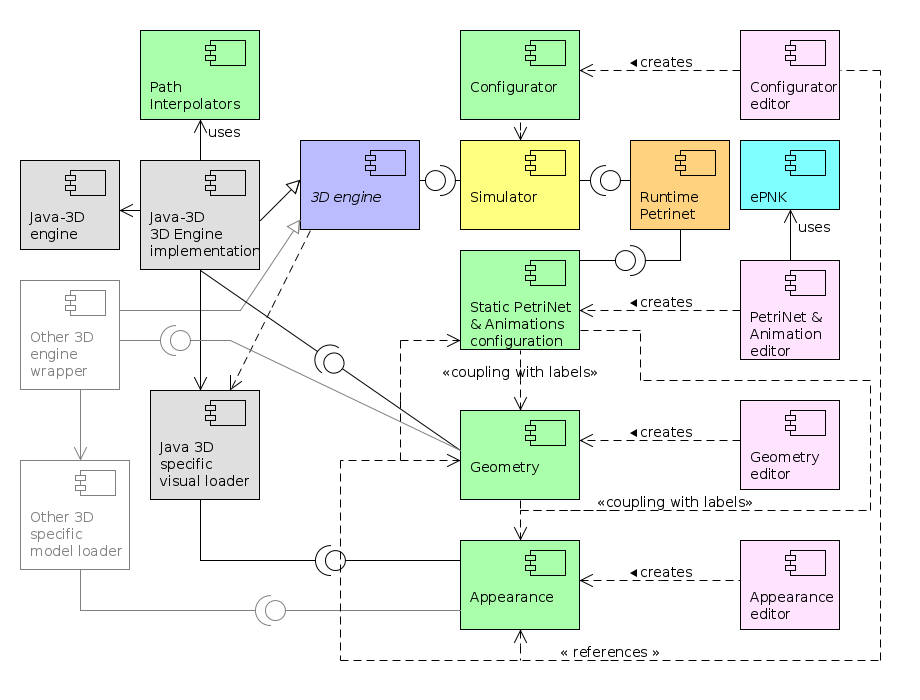
\includegraphics[scale=0.35]{image/components.png}
       \caption{Components diagram}
       \label{fig:components}	
       \end{center}
   \end{figure}

A general view of the domain model is presented in figure \ref{fig:components}. A short description of 
the most important components will be provided in the next paragraphs. More details are available
in the sections dedicated to each component. 

In order to use our system, the application user begin by using the \textbf{Petri net Editor}
to create the \textbf{Static Petri net}. When starting the \textbf{Simulator}, it would load
the \textbf{Static Petri net} and create a \textbf{Runtime Petri net}. This runtime Petri net
contains the information about Places, Arcs and Transitions, but also contains up-to-date information 
regarding the tokens present in each Place(a hash-map).

The way the tracks look like is defined in the \textbf{Geometry editor}. The settings from the geometry 
editor will be used by the 3D Engine in order to know how (on which paths) to move objects/tokens when instructed by the
Simulator. This \textbf{Geometry editor} allows the usee to create paths (curves) in the 3D space, which will
be used when animating objects during the simulation. Moreover, it allows the user to add positions on
which to place various objects(like traffic lights, trees, etc.) in the 3D space.

The 3D Engine also requires information about how the objects will look like, in order
to know how to represent tokens, tracks and other objects during the simulation. This information is set up in 
the \textbf{Appearance editor}.It is a simple editor that connects labels with 3D Models(.3ds and .obj), 
3D Shapes, Textures or Colors.

For setting up animations for the objects in the simulation we will use an \textbf{Animation Editor},
which, in our project is integrated in the Petri net editor to create an easier and more intuitive 
interface for the user. The user can set up a single animation or a sequence of animations which is
loaded by the Simator and is then used by the 3D engine to display the objects.

The \textbf{Simulator} is a component that supports the simulation of a Petri net.
In order to do so, the Simulator needs a \textbf{Petri net} to simulate, a
\textbf{3D engine} to display the simulation on and the settings provided by the \textbf{Geometry editor}, 
\textbf{Appearance editor} and the integrated \textbf{Animation Editor} to know how to map
Petri net concepts to 3D coordinates.

The \textbf{3D engine} is an abstraction of 3D engines with focus of Petri net simulations of
objects on tracks (see project definition). The idea is to facilitate various 3D engines: Java3D,
OpenGL, HTML5 without having to reimplement everything. Our system will make use of an abstract factory for
the wrapper implementations and their 3D models.

\begin{figure}[ht]
   \begin{center}
       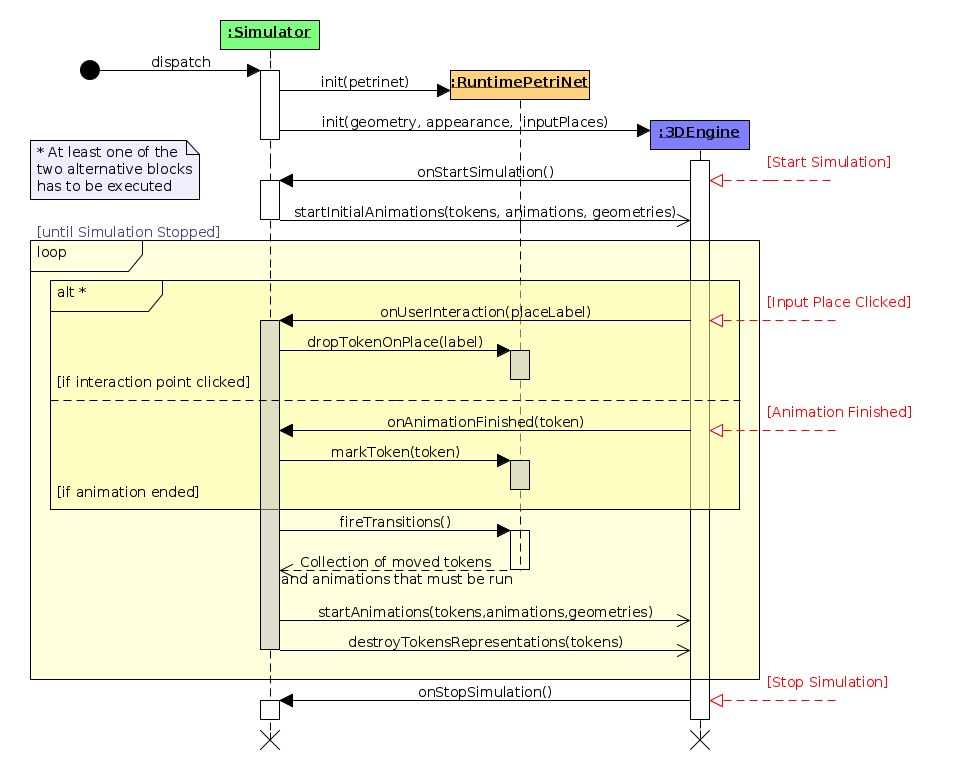
\includegraphics[scale=0.50]{image/system_sequence_diagram.png}
       \caption{System Sequence Diagram}
       \label{fig_ssd}
       \end{center}
   \end{figure}

In Figure~\ref{fig_ssd}, we represented the interaction between the main components active during a
running simulation \& visualization. The Simulator is the main component, which is started by the
user and has access to all the configuration files necessary. Then, the 3D engine is started by sending
the Geometry and Appearance configurations and the Input Places. Next, the Runtime Petri net is
initialized based on the static Petri net created by the technical user. The actual simulation is started
by the user, by clicking the Start button, event which is captured by the 3D Engine. 
The latter notifies the Simulator that the simulation was started, which, in turn, starts the
initial animations.

The simulation runs in a loop where animations are started for tokens on places. Whenever
an animation ends, the 3D Engine notifies the Simulator and the corresponding token in the Petri net
is marked as finished. If an interactive input Place has been activated (clicked upon the associated 3D Object),
then a token is created in it. In either case, the RuntimePetriNet is asked to fire any waiting
transitions \footnote{Considerations should be made on infinite loops by the technical user
configuring the network.}. A collection of moved tokens and the animations that have to be run is
returned. Using this, the Simulator might need to start new animations or to destroy representation
for tokens that do not exist in the simulation anymore\footnote{More details will be provided in
subsequent sections.}. Then the loop starts over.

The simulation stops when a special place (e.g. a Stop button) is pressed in the 3DEngine, which, in
turn, notifies the 3D Engine accordingly.

In the rest of this chapter, more details are provided for each of the components used in \epns
and general implementation details are discussed.

\subsection{Petri net Editor}
\writer{Pablo}

\index{Petri net}
\index{Petri net!Editor}
As previously stated, this component is logically separated into two parts: the Petri
net Editor itself (see figure \ref{fig:petrinet_domain_model}) and the Animation Editor
(see figure \ref{fig:animation_domain_model}). Therefore, we will describe them separately.

\index{Petri net!Domain model}
\begin{figure}[ht]
   \begin{center}
       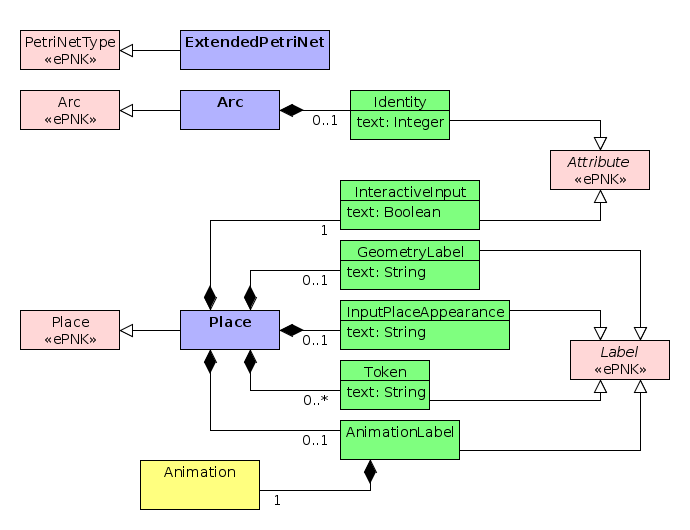
\includegraphics[scale=0.50]{image/dm_petrinet.png}
       \caption{Petri net Domain Model}
       \label{fig:petrinet_domain_model}
   \end{center}
\end{figure}

\subsubsection{ePNS Petri net classes}
\label{lst:pn_classes}
Here are described the classes that define the components of an ePNS Petri
net according to the model used for the software in development (the model is shown in
figure \ref{fig:petrinet_domain_model}).

\newpage
\textbf{Arc class} \\
The Arc class has the following attributes:
\begin{description}[labelindent=1cm]
  \item[Identity:] an ePNK Attribute with an integer that indicates the Arc's identity (used
for Token flow, for more information see "Arc Identities" in \ref{oa:generalconcepts}).
\end{description}

An Arc connects Places to Transitions and vice versa, as well as determining (thanks to
their Identity attribute) which way Tokens must go when "going through" Transitions.

\textbf{Place class} \\
The Place class has the following attributes:
\begin{description}[labelindent=1cm]
  \item[InteractiveInput:] an ePNK Attribute with a boolean value indicating whether Tokens
can be inserted into the Place (for more information see "Input Place" in \ref{oa:generalconcepts}).
  \item[GeometryLabel:] an ePNK Label with a string containing the name of the Geometry object
that will represent the Place (this will typically be a line or a point in the geometrical
description; for more information see "Track" and "SimplePosition" in \ref{arch:geometryeditor}).
  \item[InputPlaceAppearance:] an ePNK Label with a string containing the name of theAappearance
of the Place (only used if the Place is an Input Place, for more information see "Place Appearance"
in \ref{oa:generalconcepts}).
  \item[Token:] an ePNK Label representing a token with a string indicating the name of the
Appearance that will be associated to said token (for more information, see
"Token Appearance" in \ref{oa:generalconcepts}). As in classic Petri nets, a Place may contain any number of Tokens.
  \item[AnimationLabel:] an ePNK Label containing an Animation object (this will indicate the
Animation or Animation Sequence to be executed on a Token that is inserted into the Place,
whether this is through a Transition or through external means; for more information on Animations,
see "Animations" in \ref{oa:generalconcepts}).
\end{description}


\subsubsection{Animation classes}
\index{Petri net!Animation Editor}

Here are described the classes that define the animations of the
components of an ePNS Petri net for the later visualization.

\begin{figure}[ht]
   \begin{center}
       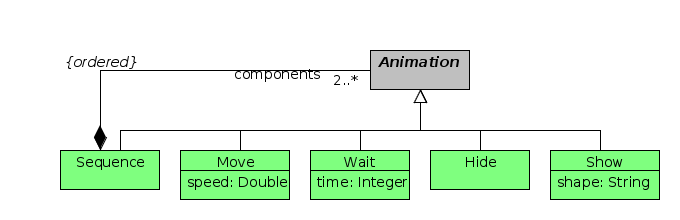
\includegraphics[scale=0.50]{image/dm_animation.png}
       \caption{Animations Domain Model}
       \label{fig:animation_domain_model}
   \end{center}
\end{figure}
  
\textbf{Animation class}

The Animation class is a definition of an animation, which will be indirectly associated to different elements of the Geometry of the Petri net and the Appearance of its components. An Animation in itself isn't anything, the classes described below are the ones that specify an Animation's behaviour.

\textbf{Sequence class}

The Sequence class is an Animation object containing:
\begin{description}[labelindent=1cm]
  \item[components]: a set of 2 or more Animation objects
\end{description}

This class is used to model an aggregation of Animations.

\textbf{Move class}

The Move class is an Animation object containing:
\begin{description}[labelindent=1cm]
  \item[speed]: Real
\end{description}

A Move object represents an animation of an object moving at a certain speed along a Track that represents the Place to which the Animation is associated.

\textbf{Wait class}

The Wait class is an Animation object containing:
\begin{description}[labelindent=1cm]
  \item[time]: Integer
\end{description}

A Wait object models an animation in which an object waits for a certain amount of time (e.g., a car waits in a crossroads for 3000 miliseconds before entering it).

\textbf{Hide class}

This object models an ``animation'' where any object currently associated to the Place to which the Animation is applied is hidden from the screen.

\textbf{Show class}

The Show class is an Animation object containing:

\begin{description}[labelindent=1cm]
  \item[shape]: String
\end{description}

This class represents the ``animation'' of showing an object (described by its shape) in the position of the Place associated to this Animation (if the Place is represented by a Track the object will be shown at the beginning of the Track). This could be used to, for example, put a traffic light into the simulation in the following way:

\begin{enumerate}
  \item Two places are created, both with the same geometrical position. One of them has attached a show(green\_light) and the other a 
  show(red\_light), where green\_light and red\_light are the appearances of a green traffic light and a red traffic light respectively.
  \item When a Token moves into one of the Places, a traffic light (a green light in one of them and a red light in the other one) would be shown.
  \item An Input Place or a Wait Animation could be used to change from a green to a red traffic light.
\end{enumerate}

%%%%%%%%%%% GEOMETRY EDITOR %%%%%%%%%%%
\subsection{Geometry editor}
\writer{Georgios}
\label{arch:geometryeditor}
The Geometry Editor is the component with which the technical user will draw the geometry on which the Petri net behavior will be simulated. This will be achieved by providing a Geometry Model that basically describes what a Geometry object is comprised of, or in other words, what the components that make up a Geometry object are.

%The technical user is the appropriate one to provide the Geometry model to the Graphical Modelling Framework (GMF). Then, the GMF will autogenerate an editor, along with other code, on which the technical user will be able to draw different geometry object, such as lines and control points. GMF is based on the Model-View-Controller (MVC) architecture and it is a core technology of the final product that the Geometry Editor will utilize.

%Figure \ref{fig:geometry_editor_structure} shows the structure of a Geometry Editor.

%\begin{figure}[ht]
%   \begin{center}
%       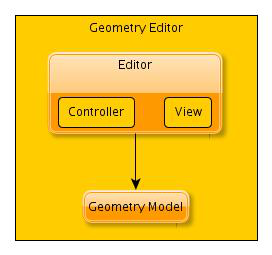
\includegraphics[scale=0.50]{image/geometry_editor_structure.png}
%       \caption{Geometry Editor Structure}
%       \label{fig:geometry_editor_structure}
%       \end{center}
%   \end{figure}

At this point the reader should recall that the simulation is track-bound. Thus, through the Geometry Editor the technical user will draw the paths (straight or curved lines-tracks) along which 3D objects will move. Furthermore, the technical user will have the possibility to set control points, such as a signals, with which the animation of the 3D objects could be controlled. Other than that, the Geometry Editor will allow for naming different geometry objects, such as tracks and signal positions. This could be achieved by a label attribute associated with every Geometry object. It constitutes a unique identifier for such an object. In this way the label attribute plays the role of one-to-one link between Places in the Perti Net and the Geometry objects. 

In particular, for visualising systems modeled as Petri nets in a track-bound manner, the Geometry model in Figure \ref{fig:geometry_domain_model} has been created.

\begin{figure}[ht]
   \begin{center}
       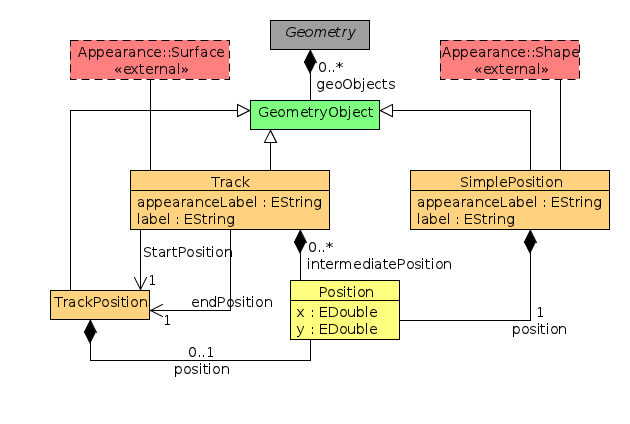
\includegraphics[scale=0.50]{image/geometry_domain_model.png}
       \caption{Geometry Domain Model}
       \label{fig:geometry_domain_model}
       \end{center}
   \end{figure}

A detailed description of each and every class in the model will be presented in that point. 

\textbf{Geometry}

The Geometry class is simply an abstract definition of a geometry. 

\textbf{GeometryObject}

The GeometryObject class is an empty class from which different geometry objects, such as Track, TrackPosition and SimplePosition, inherit. 

\textbf{Track}

A Track class consists of :
\begin{description}[labelindent=1cm]
  \item[appearanceLabel]: EString
  \item[label]: EString
\end{description}

A Track object resembles a line in the geometry. This line can be drawn between two TrackPosition objects. A Track can be either a straight or a curved line. A Track label constitutes a reference to that particular Track object while the appearanceLabel defines the appearance of the Track on hte 3D visualization space. 

\textbf{TrackPosition}

A TrackPosition is a GeometryObject that simply represents a point on a geometry. Two TrackPosition objects are needed for a Track to be created.

\textbf{Position}

A Position class contains :

\begin{description}[labelindent=1cm]
  \item[x]: EDouble
  \item[y]: EDouble
\end{description}

A Position object resembles a point in the two dimension space in a geometry. 

\textbf{SimplePosition}

A SimplePosition is a GeometryObject containing : 

\begin{description}[labelindent=1cm]
  \item[appearanceLabel]: EString
  \item[label]: EString
\end{description}

A SimplePosition object is correlated to one Position object. Its appearanceLabel defines the appearance of the SimplePosition object on the 3D visualaization space, while the label is a reference to it. 


%%%%%%%%%%% APPEARANCE EDITOR %%%%%%%%%%%
\subsection{Appearance Editor}
\index{Appearance Editor}
\writer{Jerome}
The Appearance Editor is another component we will provide to the user, allowing him to associate a visual representation to certain elements of the Petri net so each element can have a representation in the Simulator. This Editor should be used by the technical user and will be displayed as a tree. Each element of the tree will have a Label to identify it and some special properties to customize it.

We can see in Figure \ref{fig:appearance_domain_model}, the domain model associated to that component.

\begin{figure}[ht]
   \begin{center}
       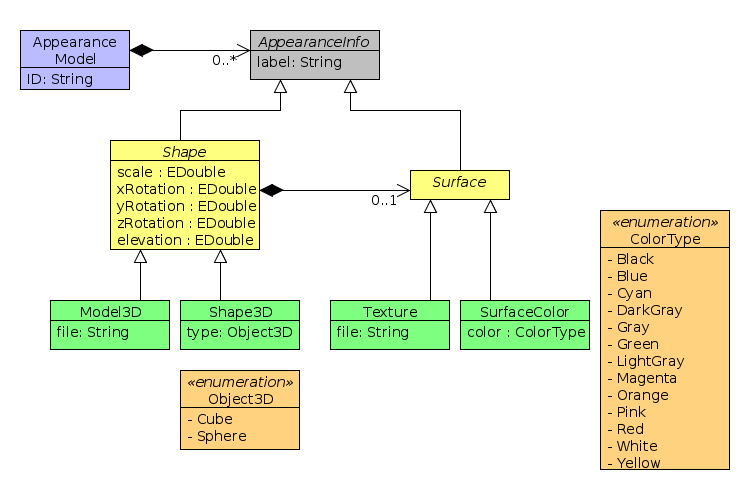
\includegraphics[scale=0.50]{image/dm_appearance.png}
       \caption{Appearance Domain Model}
       \label{fig:appearance_domain_model}
   \end{center}
\end{figure}

We will now describe in details each class of this domain model.

\textbf{Appearance Model}

The AppearanceModel class is simply an abstract definition of an appearance object. 

\textbf{AppearanceInfo}

The AppearanceInfo class is an empty class from which different appearance objects, such as Shape or Surface, inherit. 

\textbf{Shape}

A Shape class consists of :
\begin{description}[labelindent=1cm]
  \item[scale]: EDouble
  \item[xRotation]: EDouble
  \item[yRotation]: EDouble
  \item[zRotation]: EDouble
  \item[elevation]: EDouble
\end{description}

A Shape object that will be used for 3D elements. It has a lot of attributes such as scale that represents the scale the 3D object should be represented with, (x,y,z)Rotation that represent the rotation on each axe we have to apply for this object and elevation that represents the ``high'' the object has to be from the ground. This is also an abstract class and it can be inherited by the Model3D and Shape3D classes.

\textbf{Model3D}

A Model3D class consists of : 
\begin{description}[labelindent=1cm]
  \item[file]: String
\end{description}

A Model3D object contains a single proper attribute : file that represents the place of the 3D model file on the hard disk. It inherits from Shape.

\textbf{Shape3D}

A Shape3D class consists of : 
\begin{description}[labelindent=1cm]
  \item[type]: Object3D
\end{description}

A Shape3D object contains a single proper attribute : type that represents the type of 3D shape we want to load. These types are already configured internally and don't use any external 3D shape. This class inherits from Shape.

\textbf{Object3D}

An Object3D enumeration consists of :
\begin{description}[labelindent=1cm]
  \item[Cube]
  \item[Sphere]
\end{description}

An Object3D is a pre-configured 3D shape that can be used for our software. If the user wants to have another 3D shape he needs to use the Model3D object.

\textbf{Surface}

A Surface class is simply an abstract definition of a 2D object. It can be inherited from the Texture and SurfaceColor classes.

\textbf{Texture}

A Texture class consists of : 
\begin{description}[labelindent=1cm]
  \item[file]: String
\end{description}

A texture object contains a single proper attribute : file that represents the place of the Texture of the Surface on the hard disk. It inherits from Surface.

\textbf{SurfaceColor}

A SurfaceColor class consists of : 
\begin{description}[labelindent=1cm]
  \item[color]: ColorType
\end{description}

A SurfaceColor object contains a single proper attribute : color that represents the color of the Surface. This color will be one color we have pre-loadedin our software. The list of all different colors is the enumeration ColorType. This class inherits from Surface.

\textbf{ColorType}

A ColorType enumeration consists of :
\begin{description}[labelindent=1cm]
  \item[Black]
  \item[Blue]
  \item[Cyan]
  \item[DarkGray]
  \item[Gray]
  \item[Green]
  \item[LightGray]
  \item[Magenta]
  \item[Orange]
  \item[Pink]
  \item[Red]
  \item[White]
  \item[Yellow]
\end{description}

A ColorType is a pre-configured color we can use for coloring a Surface.
 
%%%%%%%%%%% CONFIGURATION EDITOR %%%%%%%%%%%
\subsection{Configuration Editor}
\writer{Ruxandra}
The Configuration Editor consists of only one class that links the Petri net,
its Geometry and its Appearance. In order to link them, the Configurator class
contains references to each of the previously mentioned classes. Also, the Configurator contains an attribute specifying the width of all the tracks in the scene. A simple
diagram that describes how the configurator gathers all the information needed
for the running simulation is shown in Figure~\ref{fig:configuration_dependencies}.

\begin{figure}[ht]
   \begin{center}
       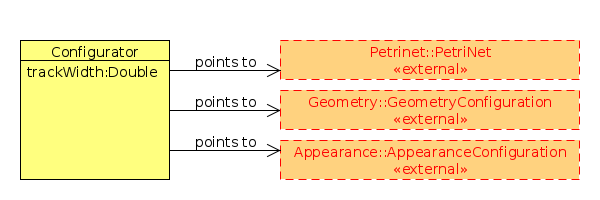
\includegraphics[scale=0.50]{image/configuration_dependencies.png}
       \caption{Configuration Dependencies}
       \label{fig:configuration_dependencies}
       \end{center}
   \end{figure}

After editing all the files, linking them in the Configurator file and setting the track width, the
simulation can be started by pressing ``Start simulator'' in the pop-up menu when right-clicking the configurator object.

\subsection{Simulator}
\index{Simulator}
\writer{Ruxandra, Marius}
The Simulator is the mediator between the RuntimePetriNet and the 3DEngine. At the initialization, it receives all the necessary data to start the simulation and the 3D visualization: the Petri net model, its geometry, its appearance and the animations associated. The simulator processes
the information received, creates a RuntimePetriNet and initializes the 3D engine with the
geometry, the appearance and the animations. It then waits for the user's input (press start button) to start the animations for the  initial tokens. The way the 3D engine and the RuntimePetriNet work will
be discussed in the next sections.

As it can be seen in figure \ref{fig:simulator_design}, the simulator implements the Engine3DListener
interface which means that it listens to the 3Dengine: it is notified when the
user start the simulation, when an animation is finished, when the user clicks
on a interactive input point or when the user stops the simulation. In each
case, it takes the appropriate measures to produce the required response.

\begin{figure}[ht]
   \begin{center}
       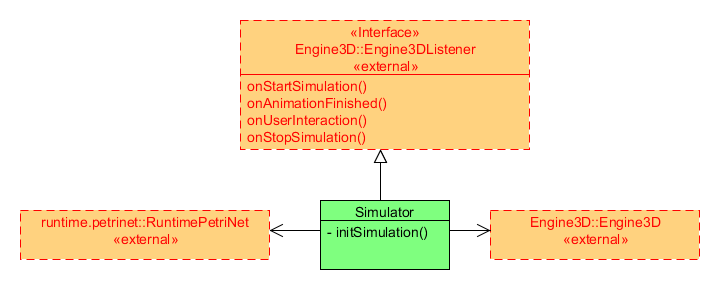
\includegraphics[scale=0.50]{image/simulator_design.png}
       \caption{Simulator with listener}
       \label{fig:simulator_design}
       \end{center}
   \end{figure}

\subsection{RuntimePetriNet}
\index{RuntimePetriNet}
\writer{Ruxandra}
The RuntimePetriNet is the component that knows where a Token is located in
the Petri net at each step of the simulation. It can be noticed that the Token
from the static Petri net is replaced in the RuntimePetriNet by a RuntimeToken,
while the Places and Transitions classes are the same. The reason for this decision
is that the places and transitions are neither created nor deleted during the
simulation(i.e. they are static components), unlike tokens, which are created
and deleted at each execution of a transition. Therefore, tokens need to be
small objects, containing just the relevant information, not all the irrelevant
information (irrelevant for the actual simulation) inherited from EMF objects.

Figure \ref{fig:petrinet_references} shows the internal structure of the RuntimePetriNet. It provides
five public methods that can be called from other classes (in our case from the
Simulator): init(), which initializes the RuntimePetriNet's structures and returns the 
movements(defined by a token and the place where the token is created) for the inital tokens; fireTransitions(), 
which iterates over all the transitions from the Petri net and executes all the ones that can be executed; fireTransition(), which
executes only one transition and returns information about the new places of tokens after executing thay transition;
markToken(), which is called whenever an animation finishes and a token needs to
be marked as finished (in order to allow previous animations to finish); getInputPlaces() which returns all
the geometry labels for the places that are defined as input places(see \ref{lst:pn_classes})

\begin{figure}[ht]
   \begin{center}
       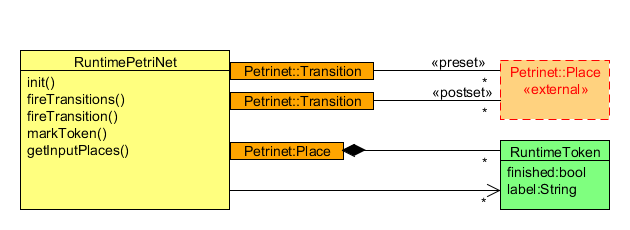
\includegraphics[scale=0.50]{image/runtime_petrinet.png}
       \caption{Runtime Petri net}
       \label{fig:petrinet_references}
       \end{center}
   \end{figure}

Structurally, the RuntimePetriNet has a dictionary that associates a place with
all the RuntimeTokens it contains, whether they are marked or not. It can be
seen in figure \ref{fig:petrinet_references} that a RuntimeToken has two main attributes : one is for
checking if the corresponding animation has finished and one for indicating the
way the RuntimeToken will look in the 3D visualization. The RuntimePetriNet
contains also two optimizations for rapidly retrieving the presets and postset
of a transition : a dictionary that associates each transition with all the
places in its preset and a dictionary that associates a transition with all the
places in its postset.

\subsection{3D Engine}
\index{3D Engine}
\writer{Cosmin}

The 3D Engine is the component of the application that handles the drawing and animation of the
objects from the simulation, on the screen. It's main responsibilities include:

\begin{itemize} 
  \item the handling of the Window in which the graphical simulation takes place
  \item handling of the buttons through which the user can interact with the simulation (Play,
  Pause, Stop)
  \item drawing the representations for the objects in the graphical visualization
  \item maintaining an association between the 3D Objects that represent the elements from the Petri
  Net and the actual Petri net objects (Tokens, Places)
  \item updating the animations according to the configurations
  \item handling user input in the case of Input Places
\end{itemize}

In order to build a system that can be easily modified, the interaction between the Simulator and
the 3D Engine is done by employing Interfaces and the Factory and Observer patterns. This
interaction can be seen in the Figure \ref{fig:engine_relations}.

\begin{figure}[ht]
   \begin{center}
       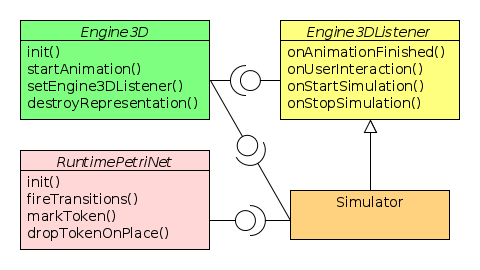
\includegraphics[scale=0.50]{image/engine_relations.png}
       \caption{3D Engine Interactions}
       \label{fig:engine_relations}
       \end{center}
   \end{figure}

The Simulator is the one that uses the Engine3DFactory to get a reference to an implementation of
the Engine3D. Then, it initializes the Engine by providing it the configurations for the Geometry
and the Appearance and registers itself as an Engine3DListener. The Engine3D keeps a reference to an
Engine3DListener (in our implementation this is the Simulator) and for every event that can occur
(e.g. an animation is finished, an user interaction has been detected, the animation was started or
stopped) it notifies it. During a normal run, when an animation is finished or an user interaction
has been detected the Engine3D notifies the Simulator using the Listener's interface and, in return,
the Simulator uses the Engine3D interface to start required animations.

Figure \ref{fig:engine_structure} shows a detailed view of \epns's implementation for the Engine3D
Interface presented above. Java 3D was chosen as the supporting 3D framework. We will now shortly
describe each of the components in the diagram and their interaction.
 
\begin{figure}[ht]
   \begin{center}
       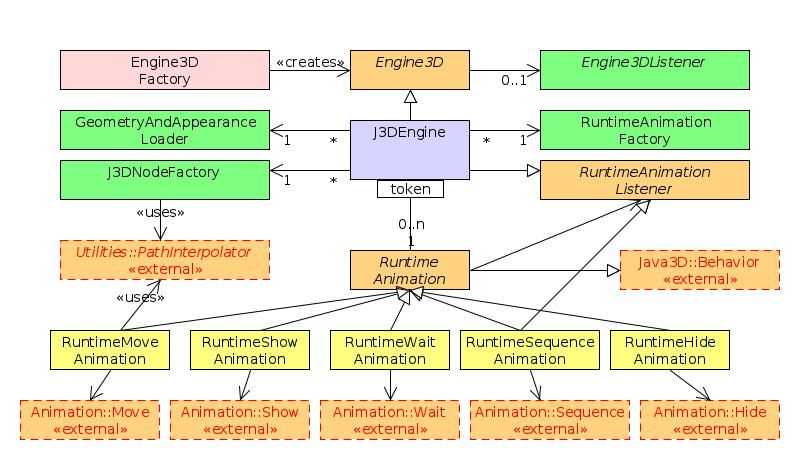
\includegraphics[scale=0.50]{image/engine_structure.png}
       \caption{3D Engine}
       \label{fig:engine_structure}
       \end{center}
   \end{figure}
   
\textbf{J3DEngine} - This class is the core implementation for our Engine3D and is handling the main
logic for the graphical representation of the simulation. Besides this, it interacts with the
Simulator, either by receiving calls (through the methods defined in the Engine3D interface) or by
sending notifications to it (through the Engine3DListener interface). Also, this class takes care of
initializing the Java 3D environment and the Window and handles user interaction.

\textbf{Engine3DListener} - As mentioned before, this is used to allow a proper mechanism for the
Engine3D to notify interested components of events regarding the simulation. As it can be seen in
Figure~\ref{fig:engine_relations}, such a listener has to implement 4 methods which allows it to be
notified when the user starts the simulation, when an animation is finished, when the user clicks on
a interactive input place or when the user stops the simulation. Using it allows the 3D Engine to
work independently of other components. For example, the J3DEngine could also be used by something
else besides the Simulator, for the purpose of animating objects.

\textbf{GeometryAndAppearanceLoader} - This helper class is initialized by the J3DEngine with the
Geometry and Appearance configurations. It loads the necessary data (e.g. textures, models etc.)
and, when required by the engine, serves geometry or appearance information.

\textbf{J3DNodeFactory} - The node factory is a Java3D dependent class, that handles the building of
the various Java3D nodes and branches, for different representations of the objects during the
visualisation. Basically, given the geometry or appearance label, it creates a new Java3D node (or
alters an existing one, if required) used for displaying objects according to the user's
preferences. For example, these nodes are used to display Token representations, visualization for
Geometry \textit{Tracks} or \textit{Simple Positions}. For the purpose of creating the tracks'
representations, the \textit{PathInterpolator} is used to compute where(position) / how(rotation)
quads should be placed to obtain a proper display result.

\index{3D Engine!Runtime Animations}
\textbf{RuntimeAnimation} - This abstract class is used by the J3DEngine to manage the animations
that are running. It holds all the required information (e.g. the RuntimeToken it is animating,
references to Java3D Nodes in the scene graph etc.). It is built as a unit that completely
self-manages its life-cycle: after it is initialized and started, all the required actions / updates
are performed automatically by it and the finalization actions \& notifications are executed
accordingly, without any other operations performed by other component (e.g. J3DEngine, Simulator).
In order to properly implement this, the Java3D \textbf{Behaviors} are used, the RuntimeAnimation
abstract class actually being an extension of the \textit{Behavior} class. What it does it that it
attaches itself to the Java3D scene graph and, based on the implementing classes (one for each
Animation - see below), it sets up wakeup conditions in order to execute code exactly when needed
(e.g. at every \textit{X} frames, after a time interval has passed etc.)

\textbf{RuntimeAnimationListener} - This interface allows the RuntimeAnimations to communicate with
other classes interested in the progress of \textbf{RuntimeAnimation}s. To exemplify, for the simple
Animations (Move, Wait, Show and Hide), the J3DEngine is used as a listener, so it is informed, for
example, when the animations are finished. However, the Sequence Animation also implements this
interface and, when executed, starts the 'child' animations by itself and registers itself as a
listener for them. Thus, when one of the animations in the sequence is finished, the next one is
started. The Sequence Animation also has to handle the proper forwarding of wakeup conditions
between the child animations and the Java 3D Engine.

\textbf{RuntimeMoveAnimation, RuntimeSequenceAnimation, RuntimeWaitAnimation, RuntimeShowAnimation,
RuntimeHideAnimation} - These 5 classes are implementations of the \textbf{RuntimeAnimation}
interface presented above and each of them takes into consideration the particularities of the
Animation type it refers to. They employ Java3D features to display the required animation or to
have the desired effects. Considering that most of the control logic is implemented in the
\textbf{RuntimeAnimation} class, these implementation mostly have to focus on the actions needed to
be performed and the next moment when they should execute actions again (see
Table~\ref{tab:runtime_animation}).

\begin{table}[ht] \centering
    \begin{tabular}{| l || l | l | } 
		\hline
		\textbf{Implementation} & \textbf{Actions} & \textbf{Next Wakeup} \\
		\hline
		Move Animation & Move the token representations & Fixed framerate \\
		Wait Animation & Just wait & Set up time interval \\
		Show Animation & Show the object & Never \\
		Hide Animation & Hide the object & Never \\
		Sequence Animation & Initialize animations and forward wakeups & When child animations require \\
		\hline
	\end{tabular}
	\caption{Table showing Runtime Animations actions and wakeups}
	\label{tab:runtime_animation}
\end{table}

\textbf{RuntimeAnimationFactory} - This class is used as a Factory class in order to initialize the
implementation for the \textbf{RuntimeAnimation} corresponding to a given \textbf{Animation}.

\subsection{Path Interpolators}
\writer{Anders}

In order to make paths in the geometry editor and their counterparts in the simulator look the same,
a utility component has been developed. As it is an architectural choice, that the simulator should
be open for new implementations of the 3D engine, it was crucial that the path interpolator component
should be independent of both GMF, EMF, and of course the chosen 3D engine. Also, not knowing the 
choice of data types in alternative 3D engines, it was chosen use \texttt{double} as the base type
for coordinates, Carthesian and polar. Another choice could have been \texttt{BigDecimal}, but knowing that 
even \textbf{Open GL} only uses float, and that BigDecimal is inefficient because of its need for garbage collection,
\texttt{double} was chosen as a fair compromise.

The path interpolators shall support the geometry editor with a list of points, that can easily be 
converted to a \texttt{PointList} without actually knowing that class. They also shall support 3D engines,
with exact position and orientation of an object at any distance from the start of a path. The two
representations shall reflect each other, even though the geometry editor does not need orientations.

Consequently two utility classes have been created: A vector (\texttt{Vector2D}) class that holds coordinates
and methods for calculating with vectors, and another class holding a vector for position and a vector for orientation.
The name of the latter class is \texttt{Where}, a name that might be changed in a later version.

The facade classes and interfaces of the path interpolator component are:

\begin{description}
  \item[\texttt{PathInterpolator}] This is the interface for interpolators in this component. It defines methods for getting the
      length of the underlying path, finding the position and orientation at any distance from the path start. These methods are 
      ment for the 3D engine to calculate where objects should be and what way they should point. I also defines a method
  	for getting intermediate point, a pixel apart, for the geometry editor. 
  \item[\texttt{Vector2D}] This is the presentation of a 2D vector. It can be used to define a position or an orientation. It supports
    Carthesian and polar coordinates. It has been developed with efficiency in mind. Many methods aim to produce as
    few new objects as possible, when making calculations.
  \item[\texttt{Where}] Is mainly a position and an orientation, implemented with two \texttt{Vector2D} fields.
    Several convenience methods are provided. 
\end{description} 

The concrete classes that implements the \texttt{PathInterpolator} interface are:

\begin{description}
  \item[\texttt{LinearPathInterpolator}] This interpolator works with straight lines, and is mainly provided as the 
    first prototype, and for testing purposes. It has also worked as a proof of concept to the \texttt{PathInterpolator}
    interface and the other facade classes.
  \item[\texttt{QuadraticBezierPathInterpolator}] This interpolator works with quadratic Bézier curves, quadratic Bézier curves
    works with two end points and an intermediate point defining the tangents to the two other points. This interpolator assumes
    that any other point is a tangent target, all other points are intermediate start/end points. In the case with an even
    number of points the last line will be straight. The code for this interpolator is \textbf{highly} inspired from the
    code in \textbf{ePNK} and uses a recursive approach.
  \item[\texttt{BezierPathInterpolator}] This interpolator uses any number of intermediate points and uses Bernstein polinominals
  	to calculate actual positions, see \ref{sec:bezier-curves} \nameref{sec:bezier-curves}.
  \item[\texttt{BezierCurvePathInterpolator}] This is a cleaned up version of \texttt{BezierPathInterpolator}. It also provides
  	extra points showing the tangents of the end points for the geometry editor.
\end{description}

The component includes additional helper classes, that can be used for other other purposes, not only in the scope of Petri net
simulations and Bézier curves. The most important are:

\begin{description}
  \item[\texttt{BezierCurve}] The \texttt{BezierCurve} class is the foundation of the \texttt{BezierCurvePathInterpolator}.
  	It incapsulates a list of \texttt{Vector2D} points and calculates the value for any $t$ $0 \leq t \and t \leq 1$ of the
  	Bézier function. It also finds the distance between two such values, and the \texttt{Where} of a distance from start $t = 0$.
  \item[\texttt{ToolBox}] The tool box is a class with static methods as the \texttt{java.lang.Math} class.
    It has methods for calculating:
    \begin{itemize}
  		\item the power of a real (\texttt{double}) number to an integer exponent. A recursive algorith is used here to increase
  		  efficiency.
  		\item the binominal coefficient of n over k. This is used by \ldots
  		\item the value of a Bernstein base polynonimal. 
	\end{itemize} 
\end{description}

\subsubsection{Bézier Curves}
\label{sec:bezier-curves}
\writer{Anders}

The most commonly known Bézier curves are quadratic and cubic Bézier curves. Quadratic Bézier curves uses three points, a start
and an end point and one intermediate point. The intermediate point determines the outgoing angle of the curve from the starting
point and the ingoing angle to the end point. The cubic Bézier curve has two intermediate points, each of them determining the 
outgoing angle of the start point and the ingoing angle of the end point, further more the distance of the intermediate points
determine the detour of the curve from start to end. Even more intermediate points can determine the detour more and more precisely.
The number of points besides the starting point, determines the order $n$ of the curve. An order $n = 1$ is a straight line,
$n = 2$ is a quadratic curve, and $n = 3$ is a cubic Bézier curve.

\begin{figure}[htp]
\begin{center}
	  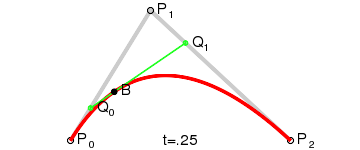
\includegraphics[scale=0.4]{image/wiki_bezier_2.png}
	  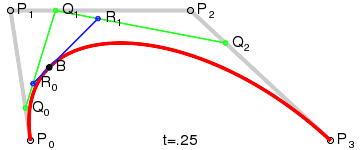
\includegraphics[scale=0.4]{image/wiki_bezier_3.png}
	  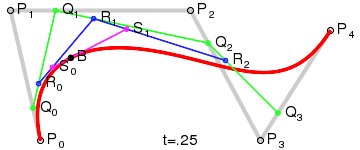
\includegraphics[scale=0.4]{image/wiki_bezier_4.png}
	  \caption{Bézier curves of order 2, 3, and 4}
	  \label{fig:wiki_bezier}
\end{center}
\end{figure}

Figure \ref{fig:wiki_bezier} shows Bézier curves of order two, three,
and four\footnote{The images has been borrowed from Wikipedia: http://en.wikipedia.org/wiki/Bézier\_curve}.
Most graphical programs doesn't use
more than third order (cubic) Bézier curves, and it is not recommended to add too many intermediate points
in the geometry editor, the curve will not be much nicer, but harder to calculate. 

In the component we use:

\begin{equation}
	B(t) = \sum_{i = 0}^n b_{i,n}(t)P_i
\end{equation}

wher $B(t)$ is the value of the Bézier function and $t \in [0,1]$. $b_{i,n}$ is the $i^{\text{th}}$ Bernstein polinomial of
degree $n$. $P_i$ is the $i^{\text{th}}$ intermediate point. The Bernstein polinomial is defined as follows:

\begin{equation}
	b_{i,n}(t) = \binom{n}{i}t^i(1-t)^{n-i}
\end{equation}

The binomial coefficient is calculated using this formula:

\begin{equation}
	\binom{n}{k} = \prod_{i = 1}^k \frac{n - k + i}{i}
\end{equation}

The implementations can be found in the \texttt{se2.e.utilities.ToolBox} class.
